
\subsection{UC21: Checkout}
\label{sec:UC21}
\begin{figure}[!ht]
    \caption{Diagramma di UC21: Checkout}
    \vspace{10px}
    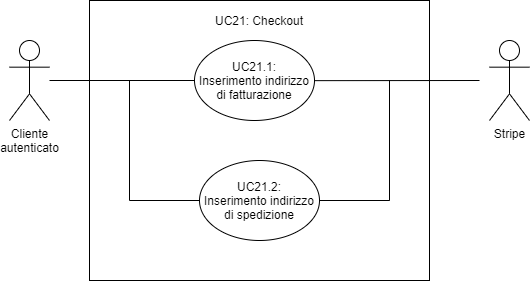
\includegraphics[scale=0.5]{../../../Images/AnalisiRequisiti/UC21}
    \centering
\end{figure}
\begin{itemize}
    \item \textbf{Descrizione:} caso d'uso per la creazione di un nuovo ordine e l'acquisto dei prodotti;
    \item \textbf{Attore Primario:} cliente autenticato;
    \item \textbf{Attore Secondario:} Stripe\textsubscript{\textbf{G}}, gestore di pagamenti di terze parti;
    \item \textbf{Precondizione:} il cliente si trova nel carrello (\hyperref[sec:UC11]{\underline{UC11}}) e ha già inserito almeno un prodotto oppure si trova nella pagina del prodotto (\hyperref[sec:UC4]{\underline{UC4}});
    \item \textbf{Input:} il cliente clicca il bottone per iniziare il checkout;
    \item \textbf{Postcondizione:} l'ordine viene emesso e aggiunto alla lista degli ordini di quel cliente; i prodotti acquistati vengono rimossi dal carrello e viene diminuita la rispettiva quantità dal deposito del venditore; il cliente viene reindirizzato alla pagina di riepilogo dell'ordine (\hyperref[sec:UC21]{\underline{UC21}});
    \item \textbf{Scenario Principale:}
          \begin{itemize}
              \item il cliente clicca il bottone per effettuare il checkout;
              \item il cliente inserisce i dati di fatturazione (\hyperref[sec:UC21.1]{\underline{UC21.1}}) e, se diversi, i dati di spedizione (\hyperref[sec:UC21.2]{\underline{UC21.2}});
              \item vengono inseriti eventuali costi di spedizione;
              \item il cliente viene reindirizzato al servizio di pagamento esterno, dove inserisce i dati di pagamento;
              \item l'ordine è emesso e segnato come completato.
          \end{itemize}
    \item \textbf{Estensioni:}
    \item Il cliente decide di non completare il checkout:
          \begin{itemize}
              \item  il cliente esce dalla pagina senza causare modifiche al carrello;
          \end{itemize}
    \item Il pagamento non è andato a buon fine:
          \begin{itemize}
              \item L'utente ritorna al carrello \hyperref[sec:UC36]{\underline{UC36}}.
          \end{itemize}
\end{itemize}

\subsubsection{UC21.1: Inserimento dell'indirizzo di fatturazione}
\label{sec:UC21.1}
\begin{itemize}
    \item \textbf{Descrizione:} Sezione per l'inserimento dell'indirizzo fatturazione;
    \item \textbf{Attore Primario:} cliente autenticato;
    \item \textbf{Precondizione:} il cliente si trova nella fase di checkout;
    \item \textbf{Input:} il cliente inserisce i dati richiesti dalla pagina;
    \item \textbf{Postcondizione:} si procede con la fase successiva del checkout (\hyperref[sec:UC21.2]{\underline{UC21.2}});
    \item \textbf{Scenario Principale:} il cliente inserisce negli appositi spazi i dati per completare l'indirizzo di fatturazione.
\end{itemize}
\subsubsection{UC21.2: Inserimento dell'indirizzo di spedizione}
\label{sec:UC21.2}
\begin{itemize}
    \item \textbf{Descrizione:} Sezione per l'inserimento dell'indirizzo spedizione;
    \item \textbf{Attore Primario:} cliente autenticato;
    \item \textbf{Precondizione:} il cliente si trova nella fase di checkout;
    \item \textbf{Input:} il cliente inserisce i dati richiesti oppure clicca un apposito bottone se l'indirizzo di spedizione è lo stesso di quello di fatturazione;
    \item \textbf{Postcondizione:} si procede con la fase successiva del checkout;
    \item \textbf{Scenario Principale:} il cliente inserisce negli appositi spazi i dati per completare l'indirizzo di spedizione oppure clicca il pulsante per autocompletarli se è il medesimo di quello di fatturazione.
\end{itemize}
\subsubsection{UC21.3: Inserimento dei dati del pagamento}
\label{sec:UC21.3}
\begin{itemize}
    \item \textbf{Descrizione:} Sezione per l'inserimento dei dati di pagamento;
    \item \textbf{Attore Primario:} cliente autenticato;
    \item \textbf{Attore Secondario:} Stripe;
    \item \textbf{Precondizione:} il cliente si trova nella piattaforma di Stripe per completare il checkout;
    \item \textbf{Input:} il cliente inserisce i dati richiesti dalla pagina;
    \item \textbf{Postcondizione:} il cliente ha inserito i dati per il pagamento;
    \item \textbf{Scenario Principale:} il cliente inserisce negli appositi spazi i dati della propria carta per il pagamento.
\end{itemize}